\documentclass{report}
\usepackage[utf8]{inputenc}
\usepackage[italian]{babel}
\usepackage{amsmath}
\usepackage{graphicx}
\usepackage{float}
\usepackage{pdfpages}
\usepackage{siunitx}

\DeclareSIUnit{\rpm}{rpm}
\sisetup{range-phrase=\div}

\title{Progetto no-brim}
\author{Daniele Moser, Francesco Maraner, Michele Mattè}



\begin{document}
\maketitle
\tableofcontents

\chapter{Introduzione}

\chapter{Meccanica}

\section{Descrizione macchina e motivazione dei componenti}
La parte meccanica, realizzata su Inventor, è stata divisa in 2 gruppi principali:
\begin{itemize}
\item Trasporto;
\item Taglio ed espulsione.
\end{itemize}

\subsection{Trasporto}
La prima parte si occupa del trasporto del tubo mediante un asse lineare ($l=\SI{300}{\mm}$) che sfrutta una trasmissione a vite a ricircolo di sfere, comandata da un motore elettrico, per spostare un pistone pneumatico (1M1), dove alla sua estremità è montata una lamiera che con la sua elasticità garantisce la corretta aderenza al tubo, sfruttando tutta la forza del pistone. Il pistone è stato collegato al pattino dell’asse lineare mediante una lamiera e una piastra. Dalla parte opposta all’asse, troviamo una lamiera a forma di “V” che garantisce il corretto scorrimento del tubo fino alla parte di taglio, grazie all’utilizzo di una rulliera costruita con dei cuscinetti a sfera.
Poco più a destra dell’asse lineare si colloca un altro pistone (2M1) fisso a telaio che si occupa di bloccare il tubo con la stessa logica del primo, contro un supporto in materiale tenero per non danneggiare l’oggetto da lavorare.
All’estremità del telaio sono presenti delle lamiere che garantiscono il corretto ingresso ed uscita del tubo dalla parte di trasporto e dei sensori per controllare la posizione di quest’ultimo. Il telaio è stato realizzato mediante l’uso di tubolari quadrati in acciaio, dove sono stati fissati i supporti per le parti nominate in precedenza.

\subsection{Taglio ed espulsione}
La seconda parte si occupa del taglio e l’espulsione del tubo mediante l’uso di una sega circolare ($D=\SI{300}{\mm}$) messa in moto da un motore elettrico monofase ($P = \SI{1,5}{\kW}$, $n_{max}=\SI{2500}{\rpm}$), il tutto collegato con una trasmissione a cinghie piatte con rapporto di trasmissione $i=\num{0.5}$ che si occupa di moltiplicare i giri della puleggia operatrice per garantire un taglio ottimale, come consigliato da tabella. Il sottoassieme descritto è stato assemblato con un “telaietto” creato con dei tubolari quadrati in acciaio di piccole dimensioni per contenere il peso complessivo (motore, trasmissione, porta cuscinetto e lama) e vincolato ad un’estremità con 2 perni (che generano un effetto cerniera) che permettono la salita e la discesa di quest’ultimo mediante un pistone a doppio effetto (3MX). Per trasformare lo spostamento lineare del pistone in angolare dovuto alla rotazione attorno ai perni sono stati montati dei perni a forcella, collocati tra una piastra fissa e la base del pistone e tra l’estremità dello stelo e il telaietto, garantendo una buona spinta senza considerevoli perdite di forze. 

Infine, troviamo l’espulsione del pezzo lavorato grazie all’utilizzo di un pistone pneumatico (4M1) dove all’estremità dello stelo è stata fissata una lamiera con delle prolunghe laterali che fanno scorrere il tubo su un piano d’appoggio (con la possibilità di essere allungato in base alla lunghezza del tubo desiderata) verso una caduta libera. Il telaio portante è stato realizzato mediante l’uso di tubolari quadrati in acciaio, dove sono stati fissati i supporti per le parti nominate in precedenza.

\section{Calcoli di progetto}
\subsection{Calcolo dei giri utili del motore}
I tubi da tagliare, utilizzati per il trasporto di fluidi possono esseri creati con 3 diversi materiali plastici:
\begin{itemize}
\item PVC (cloruro di polivinile) con	$R_m = \SI{55}{\MPa}$;
\item PVC-C $R_m = \SI{60}{\MPa}$;
\item PE (polietilene) $R_m = \SI{17}{\MPa}$;
\item PP (polipropilene) $R_m = \SI{35}{\MPa}$.
\end{itemize}
PVC, PE e PP fanno parte della famiglia dei pannelli termoplastici (tabella $V_t$ consigliate) dove la velocità di taglio $V_t$ consigliata si aggira tra $\SIrange{50}{75}{\m\per\s}$ e l’avanzamento tra $\SIrange{0.05}{0.1}{\mm\per\s}$.

\begin{figure}[H]
    \centering
    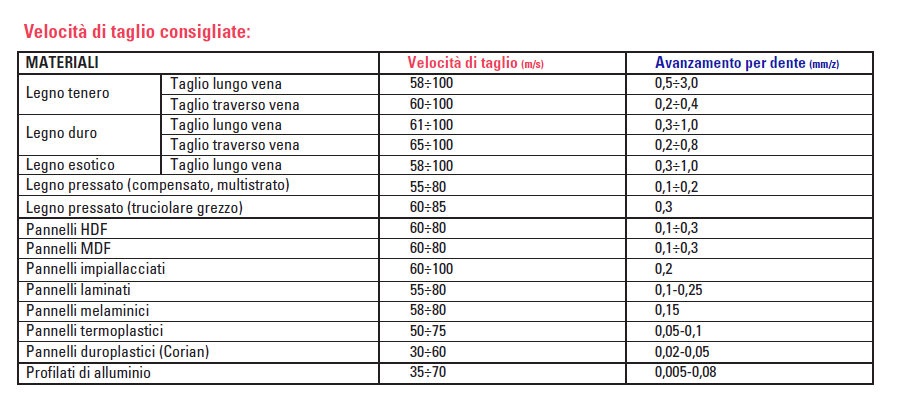
\includegraphics[width = 1\textwidth]{src/img/Vtaglio_lama.png}
    \caption{$V_t$ consigliate}
    \label{fig:vtcons}
\end{figure}

Seguendo la linea nera (per materiali plastici) della tabella, si assume un diametro della lama circolare di $D=\SI{300}{\mm}$ (inoltre utilizzata nella maggior parte dei casi, grazie al suo ottimo rapporto efficienza/ingombro).

\begin{figure}[H]
    \centering
    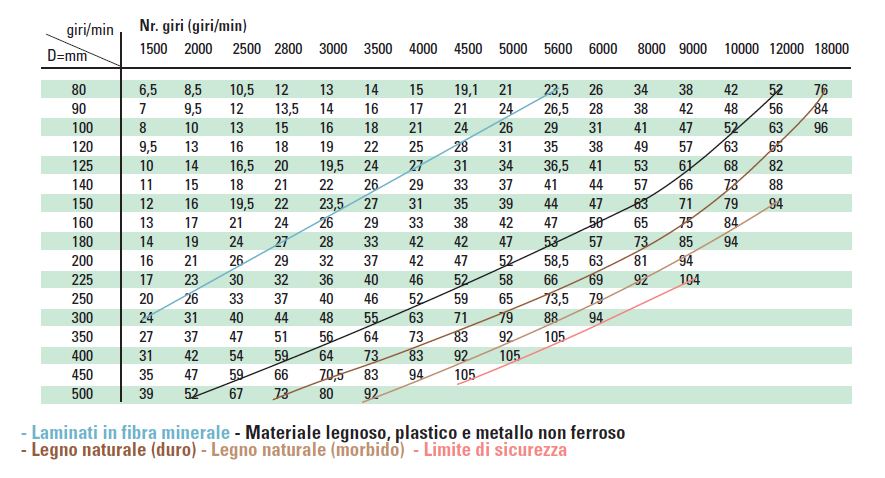
\includegraphics[width = 1\textwidth]{src/img/Vtaglio_lama_grafico.png}
    \caption{Grafico $V_t$ consigliate}
    \label{fig:grafvtcons}
\end{figure}

Conoscendo la $V_t$ richiesta dal materiale per essere tagliato possiamo calcolare il numero di giri generati dal motore, che successivamente verranno moltiplicati mediante una trasmissione a cinghie piatte.
Sapendo che:
\begin{equation}
  \omega=\frac{V_t}{r_{lama}}
\end{equation}
Si calcola:
\begin{itemize}
\item $\omega_{min} = \frac{V_t}{r} = \frac{\SI{50}{\m\per\s}}{\SI{0,15}{\m}} = \SI{334}{\radian\per\s} $;
\item $\omega_{max}  = \frac{V_t}{r}= \frac{75}{0,15} = \SI{500}{\radian\per\s}$.
\end{itemize}

Per una lettura più comoda si converte la $\omega$ in rpm mediante la seguente formula:
\begin{equation}
  n = \frac{60\omega}{2\pi}
\end{equation}

Quindi:
\begin{description}
\item $n_{min} = \frac{334\cdot 60}{2\pi} \approx \SI{3200}{\rpm}$;
\item $n_{max} = \frac{500\cdot 60}{2\pi} \approx \SI{4800}{\rpm}$.
\end{description}

Conoscendo questi dati, con l’intenzione di utilizzare una trasmissione a cinghie piatte con un rapporto di trasmissione $i = \num{0,5}$ (che moltiplica la velocità della puleggia operatrice del doppio rispetto a quella motrice) si può restringere il campo di ricerca del motore monofase fino a \SI{2500}{\rpm} massimi che, grazie alla trasmissione, potrà raggiungere i \SI{5000}{\rpm}.

\subsection{Calcolo della forza di taglio}
La taglia del tubo da tagliare, nel nostro caso, ha le seguenti dimensioni:
\begin{description}
\item $D = \SI{104}{\mm}$
\item $d = \SI{100}{\mm}$
\item $A = \SI{641}{\mm\squared}$
\end{description}

Utilizzando il carico di rottura del materiale più resistente (PVC-C) con $\sigma = \SI{60}{\MPa}$, si calcola la sua $\tau$, sapendo che $\tau = \frac{\sigma}{\sqrt{3}}$ e di conseguenza $\tau = k\frac{F}{A}$ dove per sezioni circolari $k=4/3$. Rovesciando la formula si può calcolare la $F$ necessaria per tagliare il tubo:

\begin{equation}
\tau=\frac{60}{\sqrt{3}} = \SI{35}{\MPa}
\end{equation}
\begin{equation}
F = \frac{A\tau}{k} = \SI{16,7}{\kN}
\end{equation}

\subsection{Calcolo della potenza del motore}
Per il calcolo della potenza del motore, dopo aver trovato il numero di giri necessari, è stato utilizzato il metodo sperimentale. Grazie alla presenza di una sega circolare (da falegnameria) e il tubo da lavorare, dopo varie prove e tagli siamo giunti alla conclusione di adottare un motore con una potenza di \SI{1,5}{\kW}. La possibilità di provare il taglio ci ha permesso di stabilire le seguenti considerazioni:
\begin{itemize}
\item Le velocità di taglio, calcolate in precedenza sono state del tutto coerenti con le prove effettuate.
\item La velocità di avanzamento, invece, ha soddisfatto le aspettative con un andamento lento e costante, senza imprimere troppa forza (circa \SI{50}{\N}) tra il tubo e la lama per evitare che quest'ultima si bloccasse.
  \end{itemize}
\subsection{Dimensionamento della trasmissione}
Le cinghie sono organi flessibili impiegati nella trasmissione di potenza da una puleggia motrice a una condotta, montate su alberi disposti ad una certa distanza (interasse). Le cinghie possono appartenere a due gruppi distinti: cinghie di tipo convenzionale e cinghie sincrone.
Le cinghie di tipo convenzionale trasmettono il moto sfruttando l’aderenza (attrito) con il profilo esterno della puleggia. In questo caso possono verificarsi scorrimenti fra la cinghia e la puleggia durante il moto.
Le cinghie sincrone trasmettono il moto tramite l’ingranamento dei denti della cinghia con quelli della puleggia. Non sono soggette a scorrimento e necessitano di un precarico molto modesto.
Industrialmente sono usate cinghie piatte, trapezoidali e sincrone.
Per dimensionare una trasmissione partiamo dai dati del motore, forniti dal datasheet:

\begin{table}[H]
\centering
\begin{tabular}{|l|c|}
\hline
\multicolumn{2}{|c|}{\textbf{Dati motore}} \\ \hline
Potenza & \SI{1,5}{\kW} \\ \hline
Giri motore & \SI{2500}{\rpm} \\ \hline
Diametro albero & \SI{19}{\mm} \\ \hline
\end{tabular}
\end{table}

Successivamente, una volta trovato il numero di giri che vogliamo sviluppare sull’operatrice ($n=\SI{5000}{\rpm}$), calcolo il rapporto di trasmissione ($i$) e l’interasse ($I$) tra i due elementi rotanti in base alla dimensione delle mie pulegge, che assumo a piacere dalla serie di Renard R20 a partire da un diametro minimo di \SI{40}{\mm}.

Assumiamo il diametro della puleggia motrice $D_m=\SI{100}{\mm}$ e di conseguenza (per rispettare il rapporto di trasmissione e la serie R20) $D_o=\SI{50}{\mm}$ per il diametro dell’operatrice. Questa scelta è giustificata dagli ingombri in fase di modellazione 3D per tagliare correttamente il tubo senza urti.
Il calcolo dell’interasse dipende dal carico, nel nostro caso $I\geq 3\cdot D_m$ per trasmissioni a carico variabile. Una volta rispettata questa condizione si può scegliere a piacimento la lunghezza in base alle esigenze (ingombri, etc...)

\begin{table}[H]
\centering
\begin{tabular}{|l|c|l|}
\hline
\multicolumn{2}{|c|}{\textbf{Dati Pulegge}} & \multicolumn{1}{c|}{\textbf{Formula}} \\ \hline
Numero giri motrice ($n_m$) & \SI{2500}{\rpm} & Fornito dal motore \\ \hline
Numero giri operatrice ($n_o$) & \SI{5000}{\rpm} & $\frac{n_m}{i}$ \\ \hline
Rapporto di trasmissione ($i$) & \num{0,5} & $\frac{n_m}{n_o}$ \\ \hline
Diametro puleggia motrice ($D_m$) & \SI{100}{\mm} & Scelta personale rispettando R20 \\ \hline
Diametro puleggia operatrice ($D_o$) & \SI{50}{\mm} & $D_o=D_m\cdot i$ \\ \hline
Interasse ($I$) & \SI{300}{\mm} & $I=3\cdot D_m$ \\ \hline
\end{tabular}
\end{table}

Durante la progettazione di una trasmissione è importante consultare le tabelle unificate che forniscono dati di correzione in base ai materiali utilizzati per la realizzazione e il servizio che devono compiere.
Dati provenienti dalle tabelle del manuale di Meccanica:
\begin{table}[H]
\centering
\begin{tabular}{|c|c|l|}
\hline
\multicolumn{2}{|c|}{\textbf{Dati tabelle}} & \multicolumn{1}{c|}{\textbf{Provenienza dati}} \\ \hline
$F_s$ & \num{1,2} & Tab. I.101 Fattore di servizio \\ \hline
$F_t$ & \num{1} & Tab. I.102 Fattore correttivo \\ \hline
$F_\alpha$ & \num{1} & Tab. I.108 Coeff. correzione \\ \hline
$P_1$ & \num{0,7} & Tab. I.106 P specifica (cinghia gomma-tessile) \\ \hline
\end{tabular}
\end{table}

\subsubsection{Calcolo della potenza corretta}
\begin{equation}
P_c=P\cdot F_s\cdot F_t
\end{equation}
Dove $P$ è la potenza erogata dal motore, $F_s=\num{1,2}$ da tabella per macchine utensili che lavorano dalle 8 alle 10 ore al giorno e $F_t=1$ da tabella per condizioni normali.
\begin{equation}
P_c = \SI{1,5}{\kW}\cdot \num{1,2}\cdot 1 = \SI{1,8}{\kW}
\end{equation}
\subsection{Calcolo della velocità periferica della puleggia minore}
\begin{equation}
  V = \frac{\pi D_{min}n_{min}}{\num{60000}}
\end{equation}
Dove $D_{min}=D_o$ e $n_{min}=n_o$.
\begin{equation}
V=\frac{\pi\cdot 50\cdot 5000}{\num{60000}} = \SI{13,1}{\m\per\s}
\end{equation}

\subsubsection{Calcolo della lunghezza della cinghia}
\begin{equation}
  l=2I+\frac{\pi (D_m+D_o)}{2}+\frac{(D_o-D_m)^2}{4I}=\SI{838}{\mm}\approx\SI{840}{\mm}
\end{equation}
Si approssima a \SI{840}{\mm} per lasciare un po' di gioco prima di tendere o allentare la cinghia.

\subsubsection{Calcolo dell’angolo di avvolgimento $\alpha$}
\begin{equation}
  \alpha = \SI{180}{\degree}-\SI{57}{\degree}\cdot\frac{D_m-D_o}{I}=\SI{190}{\degree}
\end{equation}
Il valore servirà per trovare $F\alpha$ da tabella.
\subsubsection{Calcolo della larghezza della cinghia $a$}
I principali materiali utilizzati per la costruzione di cinghie piatte sono:
\begin{itemize}
\item cuoio;
\item struttura composita di laminati plastici e gomme o resine;
\item struttura composita di gomme e tessili;
\item cotone, balata e altre fibre tessili vegetali;
\item gomma o materiali plastici (per alte velocità).
\end{itemize}
Da questa informazione si può calcolare la larghezza della cinghia ricavando il valore $P_1$ in base al materiale scelto, nel nostro caso gomma-tessile pesante in cotone a 4 tele, data la seguente formula:
\begin{equation}
  a = \frac{P_c}{P_1F_\alpha}=\frac{\SI{1,8}{\cm}}{\SI{0,7}{\cm}\cdot 1} = \SI{2,57}{\cm}\approx\SI{26}{\mm}
\end{equation}
La larghezza della cinghia è stata scelta in riferimento ai valori dati dalla serie R40, a partire dal valore minimo di 16 mm.

\subsubsection{Calcolo dello spessore della cinghia $s$}
Dalla seguente tabella ricavo lo spessore $s$ della cinghia in base al materiale scelto in precedenza. In questo caso \SI{6}{\mm}.
\begin{figure}[H] % per inserire l'immagine subito sotto il testo
    \centering
    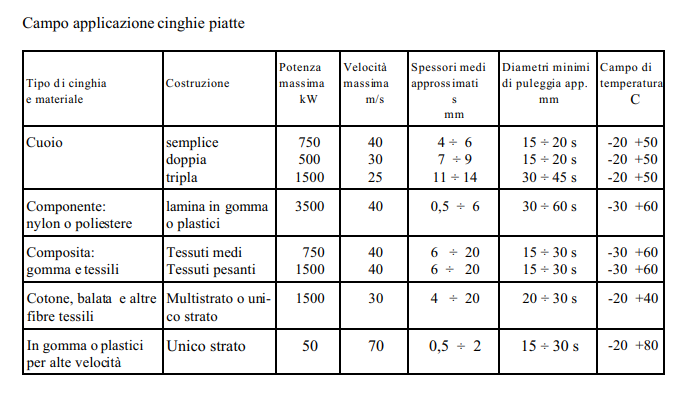
\includegraphics[width=1\textwidth]{src/img/tabella_cinghie.png}
    \caption{Parametri consigliati per vari tipi di cinghie}
    \label{fig:cinghie}
\end{figure}

\subsubsection{Calcolo della larghezza della puleggia $b$}
\begin{equation}
  b = a\num{1,15}\approx\SI{30}{\mm}
\end{equation}
\subsubsection{Calcolo della bombatura della puleggia $h$}
Le pulegge per cinghie piatte vengono costruite con profilo esterno leggermente bombato per ottenere la stabilità della cinghia sulla corona. I materiali più indicati sono l’alluminio, per il peso contenuto, o la ghisa per piccole serie.
\begin{equation}
 h=b\num{0,006}=\SI{0.186}{\mm}
\end{equation}
\section{Schema elettropneumatico}
\subsection{Scelta dei componenti}
Lo schema elettropneumatico è stato realizzato con i seguenti componenti:
\begin{description}
\item[Compressore] Si occupa di accumulare e innalzare la pressione dell’aria all’interno del suo serbatoio per alimentare il circuito pneumatico;
\item[Gruppo trattamento aria] Composta da filtro di scarico manuale, un riduttore di pressione variabile, un manometro e una valvola di sicurezza (quasi sempre inclusa nei gruppi trattamento aria industriali per togliere aria al sistema in caso di emergenza);
\item[Pistone pinza mobile 1M1, pistone pinza fissa 2M1, pistone espulsore 4M1] Composti dalla stessa logica, tramite l'uso di:
  \begin{itemize}
  \item 1 pistone a singolo effetto con ritorno a molla con le seguenti caratteristiche: corsa di \SI{50}{\mm}, diametro pistone \SI{16}{\mm} e forza di spinta teorica a $\SI{6}{\bar}$ di $F=\SIrange{90}{120}{\bar}$ (dove la sola andata è utile per svolgere il lavoro richiesto di bloccaggio ed espulsione);
  \item 1 strozzatore che si utilizza solamente uno strozzatore senza una o più valvole di non ritorno perché la regolazione della portata mediante strozzatura su ambedue i lati viene spesso applicata in cilindri a semplice effetto o in cilindri di piccole dimensioni che svolgono lavori “semplici”. Quest’aspetto inoltre va a vantaggio dei costi di realizzazione dell’impianto e della semplicità d’applicazione;
  \item 1 valvola 3/2 normalmente chiusa comandata elettricamente nella fase di spinta e con ritorno a molla;
  \end{itemize}
\item[Pistone sollevamento lama circolare 3MX] Composto da:
  \begin{itemize}
  \item 1 pistone a doppio effetto con le seguenti caratteristiche: corsa \SI{100}{\mm}, diametro del pistone \SI{32}{\mm} e forza di spinta teorica a \SI{6}{\bar} di $F=\SIrange{415}{483}{\N}$, dati necessari a soddisfare il corretto movimento della lama verso l'alto, considerando che il peso che deve movimentare è composto dal telaietto con relativa trasmissione (motore, cinghia, pulegge etc) che risulta essere circa \SI{25}{\kg}, di conseguenza \SI{250}{\N} con un ulteriore aggiunta di \SI{50}{\N} per la fase di avanzamento come descritto nei calcoli. In questo modo, con una determinata forza richiesta ($F=\SI{300}{\N}$) è stato scelto un pistone leggermente sovradimensionato per tenere conto delle possibili piccole perdite di forza dovute agli attriti dei perni a forcella;
  \item 2 strozzatori in scarico per ottenere una buona regolazione della portata, entro certi limiti indipendenti dal carico applicato allo stelo, poiché viene guidato dal cuscino d’aria che si forma nella camera di scarico; agendo sulle viti di regolazione degli strozzatori si possono tarare separatamente le velocità delle due corse.
  \item 1 valvola 5/3 a centri chiusi comandata elettricamente con ritorno a molla in ambedue i versi di commutazione per comandare il pistone a doppio effetto. La scelta di questa valvola è dovuta alla necessità di mantenere in posizione la lama (senza spostarsi in punti indesiderate, evitando danni all’oggetto da tagliare) in caso di arresto voluto o improvviso.
  \end{itemize}

\item[Finecorsa dei pistoni] Festo prevede l’utilizzo di sensori magneti che determinano la corsa dello stelo, montati direttamente sul cilindro.
\end{description}

\subsection{Lista componenti}
\begin{table}[H]
\centering
\begin{tabular}{|l|c|}
  \hline
  {\textbf{Componenti}} & \textbf{Quantità} \\ \hline
  Pistone sing. effetto & 3 \\ \hline
  Pistone doppio effetto & 1 \\ \hline
  Elettrovalvola 3/2 nc con ritorno a molla & 3 \\ \hline
  Elettrovalvola 5/3 centri chiusi con ritorno a molla & 1 \\ \hline
  Strozzatori & 5 \\ \hline
  Valvole di non ritorno & 2 \\ \hline
  Gruppo trattamento aria & 1 \\ \hline
  Compressore & 1 \\ \hline
\end{tabular}
\end{table}

\section{Elettronica}
% PCB e quadro elettrico
\chapter{Parte Elettronica}

\section{Descrizione circuiti e motivazione dei componenti}

La parte elettronica, realizzata utilizzando Kicad e DesignSpark Eletrical, è stata suddivisa in 2 parti separate: 

\begin{description}
\item \textbf{PCB}. La prima parte è costituita da una serie di circuiti che permettono ad Arduino di comandare 4 elettrovalvole e due motori rispettivamente da 24V e da 230V.
Nel caso specifico viene inserito tra l'output di Arduino e l'elettrovalvola, un Mosfet che fungerà da interuttore per alimentare e disalimentare l'elettrovalvola in questione o il motore.
Per quanto riguarda le dimensioni del circuito stampato risultano contenute nonostante la quantità di dispositivi ad esso collegati, infatti il circuito integrea solamente la parte composta da una morsettiera con 10 connettori, dedicati ad ognuno degli ingressi necessari, i circuiti di comando e i morsetti di uscita.

Ogni circuito di comando è composto un mosfet e un diodo: 
\begin{description}
\item La funzione del diodo in questo circuito è quella di proteggere il mosfet e l'uscita di Arduino da sovratensioni indesiderate provocate dagli avvolgimenti presenti nelle elettrovalvole e nei motori, in alcuni casi viene inserito anche pèer evitare le invesioni di tensione.
Per quanto riguarda il circuito di comando per il motore monofase 230v, utilizzato per la sega, si è preferito introdurre anche un relè così da permettere di utilizzare un mosfet con corrente di sollecitazione minore e ridurre la tensione massima presente sulla scheda da 230v DC a "soli 24v" DC.
\item Il mosfet è il cuore del circuito, infatti può essere visualizzato come un rubinetto che grazie ad una piccola sollecitazione(0-10mA) riesce a veicolare correnti di valore molto più alte (1-2A), nel nostro caso le correnti non superano i 2A, quest'ultimi date le correnti basse non necessitano della presenza di una qualsiasi aletta di raffreddamento. 
\end{description}

\section{Programmazione}
% Schema a blocchi del sistema
% Spiegazione programma
% Ciclogramma

\section{Utilizzo della macchina}

\section{Sviluppi futuri}

\section{Crediti}


\end{document}